\begin{frame}[t,allowframebreaks, allowdisplaybreaks]
    \subsubsection{Insert}
    \frametitle{B-Tree Operations---Insert Value}
    \begin{columns}
        \begin{column}{\textlecolumn}
            \begin{block}{}
                \begin{itemize}
                    \item The insertion algorithm in the B-Tree almost has nothing to share with any tree insertion algorithm.
                    \item The first section of the code is the same \lstinline|find| algorithm so we can see if the value to add is already 
                        stored in the B-Tree and where could it be stored, also storing in a stack the nodes that we are going to access.
                    \item Then, if the node isn't full yet, we are just going to move everything by an index until the current elements are 
                        less than the key that we are going to insert.
                    \item But, if the node is full, we will get a new node for the B-Tree and split in half the full node.
                    \item Then, insert the new key into one of thoose of the splited nodes.
                    \item Then, the median key of the splited node will be taken from the nodes and will be inserted on the upper node.
                    \item In the new insertion of the median key and new node, will be repeated until we have a non-full node which can 
                        take another element, or if we reach the root node we will have to do a extra process.
                    \item This extra process is that we have to split the root node, create a new node and increase the height of the B-Tree by inserting the new node with 
                        keys, pointers and such to the rest of the B-Tree above everything.
                    \item \textbf{This is one of the only ways that the B-Tree can change it's height.}
                \end{itemize}
            \end{block}
        \end{column}
        \begin{column}{\textricolumn}
        \end{column}
    \end{columns}
    
    \framebreak{}

    \inputminted[
        highlightlines={13, 14, 17, 20, 26, 30, 31, 33, 35, 38, 42, 45, 56, 64, 65, 66, 67, 81, 98, 99, 100, 102, 103, 104, 108, 110, 111, 117, 119, 121, 122, 123, 124, 125, 126, 130, 131},
    ]{c}{resources/code/b_tree_insert.c}

    \begin{figure}[h!]
        \includegraphics[%
            width=0.45\linewidth,%
            page=1%
        ]{resources/made/B-Trees_insert_example.pdf}
    \end{figure}

    \begin{itemize}
        \item Now, lets create a new empty tree and insert a lot of elements in a \(t\left(2, 0\right)\) B-Tree. With the bounds \(\alpha\) and \(2\alpha - 1\).
    \end{itemize}
\end{frame}
